% =====================================================================
% Differentiable Chebyshev-NUFFT Hybrid Layer for Physics-Informed
% Neural Networks with Non-Periodic Boundary Conditions
%
% Target: Journal of Scientific Computing (JSC), Springer
% Template: sn-jnl (Springer Nature), sn-mathphys reference style
% Authors: Fuchang Wang (Emergency Management University),
%          Huirong Cao (Langfang Normal University)
% =====================================================================

\documentclass[sn-mathphys,Numbered]{sn-jnl}

%%% Packages %%%
\usepackage{graphicx}
\usepackage{multirow}
\usepackage{amsmath,amssymb,amsfonts}
\usepackage{amsthm}
\usepackage{mathrsfs}
\usepackage[title]{appendix}
\usepackage{xcolor}
\usepackage{textcomp}
\usepackage{booktabs}
\usepackage{algorithm}
\usepackage{algorithmicx}
\usepackage{algpseudocode}
\usepackage{geometry}
\usepackage{manyfoot}
\usepackage{hyperref}
\usepackage{caption}
\usepackage{subcaption}
\usepackage{siunitx}

%%% Theorem environments (sn-jnl defines thmstyleone/two/three) %%%
\theoremstyle{thmstyleone}
\newtheorem{theorem}{Theorem}
\newtheorem{proposition}[theorem]{Proposition}
\newtheorem{lemma}[theorem]{Lemma}
\newtheorem{corollary}[theorem]{Corollary}

\theoremstyle{thmstyletwo}
\newtheorem{example}{Example}
\newtheorem{remark}{Remark}

\theoremstyle{thmstylethree}
\newtheorem{definition}{Definition}

%%% Hyperref setup %%%
\hypersetup{colorlinks=true, linkcolor=blue, citecolor=blue, urlcolor=blue}

%%% New commands %%%
\newcommand{\R}{\mathbb{R}}
\newcommand{\C}{\mathbb{C}}
\newcommand{\N}{\mathbb{N}}
\newcommand{\dd}{\mathrm{d}}
\newcommand{\T}{\mathsf{T}}
\newcommand{\calD}{\mathcal{D}}
\newcommand{\calL}{\mathcal{L}}
\newcommand{\calN}{\mathcal{N}}
\newcommand{\calO}{\mathcal{O}}
\newcommand{\calB}{\mathcal{B}}
\newcommand{\bftheta}{\boldsymbol{\theta}}
\newcommand{\bfx}{\boldsymbol{x}}
\newcommand{\bfk}{\boldsymbol{k}}
\newcommand{\cheb}{\mathrm{cheb}}
\newcommand{\nufft}{\mathrm{nufft}}
\newcommand{\hybrid}{\mathrm{hybrid}}

\raggedbottom

\begin{document}

%%% =====================================================================
%%% Title and Authors
%%% =====================================================================
\title[Differentiable Chebyshev--NUFFT Hybrid Layer]
{Differentiable Chebyshev--NUFFT Hybrid Layer for Physics-Informed Neural Networks with Non-Periodic Boundary Conditions}

\author*[1]{\fnm{Fuchang} \sur{Wang}}\email{wangfuchang@cidp.edu.cn}
\author[2]{\fnm{Huirong} \sur{Cao}}\email{huirongcao@126.com}

\affil*[1]{\orgdiv{College of Science}, \orgname{Emergency Management University},
  \orgaddress{\street{No. 456 College Road}, \city{Sanhe}, \postcode{065201},
  \state{Hebei}, \country{China}}}

\affil[2]{\orgdiv{College of Science}, \orgname{Langfang Normal University},
  \orgaddress{\street{No. 100 Ai-min Road}, \city{Langfang}, \postcode{065000},
  \state{Hebei}, \country{China}}}

%%% =====================================================================
%%% Abstract
%%% =====================================================================
\abstract{
We propose a differentiable hybrid spectral layer for computing spatial derivatives in physics-informed neural networks (PINNs) on non-periodic domains with arbitrary collocation point distributions. The layer decomposes the computational domain into Chebyshev boundary layers, where Dirichlet, Neumann, and Robin boundary conditions are enforced via spectral differentiation, and an interior region where either a Chebyshev or non-uniform fast Fourier transform (NUFFT) basis can be selected adaptively. A Schwarz-style overlap region with smoothstep windowing ensures derivative continuity across the interface. Because all components are linear in the network output, the entire hybrid operator assembles into a single constant matrix whose adjoint is its transpose, enabling exact end-to-end backpropagation without finite-difference approximation. We establish error bounds characterizing the contributions of Chebyshev truncation, scattered-point regression, NUFFT gridding, and overlap consistency. Numerical experiments on one- and two-dimensional Poisson equations with Dirichlet, Neumann, and Robin boundary conditions, as well as a one-dimensional heat equation, demonstrate that the proposed method achieves accuracy comparable to automatic-differentiation-based PINNs ($4.8\times10^{-6}$ in 1D, $9.9\times10^{-6}$ in 2D) while training $1.6$--$2.8\times$ faster, and that pure Fourier methods fail to converge on non-periodic problems, confirming the necessity of the Chebyshev boundary treatment.
}

\keywords{Physics-informed neural networks \sep Spectral methods \sep Chebyshev polynomials \sep
Non-uniform FFT \sep Differentiable programming \sep Non-periodic boundary conditions \sep
Adjoint method}

\maketitle

%%% =====================================================================
%%% 1. Introduction
%%% =====================================================================
\section{Introduction}\label{sec:intro}

\subsection{Background and motivation}
Physics-informed neural networks (PINNs), introduced by Raissi et al.~\cite{raissi2019physics}, embed partial differential equations (PDEs) into the loss function of a neural network, providing a mesh-free framework for solving forward and inverse problems. The canonical PINN computes spatial derivatives of the network output via automatic differentiation (AD), which is flexible but suffers from two well-known limitations in scientific computing: (i) AD scales poorly with the order and dimensionality of derivatives, requiring repeated backward passes that dominate training time for high-order or multi-dimensional PDEs; and (ii) AD-derived derivatives inherit the approximation error of the neural network, potentially compromising the high-order accuracy that classical spectral methods achieve for smooth solutions.

Spectral methods~\cite{trefethen2000spectral,boyd2001chebyshev,canuto2006spectral} offer an attractive alternative: by representing functions in a suitable basis (Fourier for periodic domains, Chebyshev for non-periodic domains), derivatives can be computed with spectral (exponential) convergence for analytic solutions. Recent work~\cite{wang2026differentiable} has demonstrated that embedding a differentiable non-uniform fast Fourier transform (finufft) layer into PINNs enables spectral-accuracy derivative computation on arbitrary non-uniform collocation points, significantly outperforming AD-based PINNs on periodic problems. However, this approach is inherently limited to periodic boundary conditions, as the Fourier basis assumes periodic extension of the solution.

Many important PDEs in scientific computing and engineering are posed on non-periodic finite domains with Dirichlet, Neumann, Robin, or mixed boundary conditions. For such problems, Chebyshev spectral methods are the standard choice, owing to their ability to handle general boundary conditions and their exponential convergence for analytic solutions on finite intervals. The challenge lies in combining the boundary-condition flexibility of Chebyshev methods with the non-uniform sampling capability of NUFFT within a single differentiable layer.

\subsection{Related work}
Our work intersects several active research areas.

\paragraph{Differentiable spectral operators.}
Fourier neural operators (FNO)~\cite{li2021fourier} and physics-informed neural operators (PINO)~\cite{li2024pino} employ spectral convolution in Fourier space, but require uniform grids and assume periodicity. Fourier continuation (FC) methods~\cite{maust2022fc,bruno2020fc} extend non-periodic functions to periodic ones by solving small linear systems near boundaries, enabling FFT-based differentiation; FC-PINO~\cite{maust2022fc} applies this idea to neural operators. However, FC methods remain on uniform grids and incur the cost of solving extension systems. Lingsch et al.~\cite{lingsch2024beyond} extend Fourier-based neural operators to arbitrary point distributions via direct spectral evaluation, but retain the periodic complex-exponential basis and do not handle non-periodic boundary conditions.

\paragraph{Chebyshev neural methods.}
Spectral neural operators (SNO)~\cite{fanaskov2022sno} use Chebyshev and Fourier series expansions in coefficient space. Chebyshev spectral neural networks (CSNN)~\cite{yin2024csnn} construct single-layer networks with Chebyshev basis functions satisfying boundary conditions. Orthogonal polynomial neural operators (OPNO)~\cite{liu2022opno} rigorously enforce Dirichlet, Neumann, and Robin conditions via orthogonal polynomial bases. SEDONet~\cite{abid2025sedonet} embeds Chebyshev spectral dictionaries into DeepONet inputs. All these methods operate on uniform or regular collocation nodes and do not support arbitrary non-uniform point distributions.

\paragraph{Non-uniform point differentiation in PINNs.}
DT-PINN~\cite{sharma2022dt} and RBFDQ-PINN~\cite{xiao2024rbfdq} use radial-basis-function finite differences for derivative computation on non-uniform points, achieving only local (polynomial-order) accuracy. Spectral PINNs~\cite{yu2024fourier,lin2022nfs} use Fourier spectral differentiation but require uniform grids or interpolation. To our knowledge, no existing method combines global spectral accuracy, non-uniform collocation support, and rigorous non-periodic boundary condition handling in a single differentiable layer.

\subsection{Contributions}
This paper makes the following contributions:

\begin{enumerate}
    \item \textbf{Differentiable Chebyshev spectral layer}: We implement a fully differentiable Chebyshev differentiation layer based on Gauss--Lobatto differentiation matrices, with exact adjoint (matrix transpose) for backpropagation. The layer supports arbitrary domains and Dirichlet, Neumann, and Robin boundary conditions through boundary-degree-of-freedom elimination.

    \item \textbf{Chebyshev--NUFFT hybrid architecture}: We design a domain decomposition framework that uses Chebyshev differentiation in boundary layers (where non-periodic boundary conditions are enforced) and an adaptive interior basis (Chebyshev for non-periodic accuracy, NUFFT for periodic subdomains or uniform sampling). A Schwarz-style overlap region with smoothstep windowing ensures derivative continuity, and the entire operator assembles into a single constant matrix for efficient training.

    \item \textbf{Exact adjoint derivation and error analysis}: We rigorously derive the adjoint operator of the hybrid layer, composing the adjoints of the Chebyshev differentiation matrix, NUFFT Type~1/Type~2 transforms, interpolation operators, and window functions. We establish error bounds decomposing the total error into Chebyshev truncation error, NUFFT gridding error, and overlap interpolation error, with convergence rates for analytic solutions.

    \item \textbf{Comprehensive numerical validation}: We validate the method on 1D and 2D Poisson equations with Dirichlet, Neumann, and Robin boundary conditions, a 1D heat equation, and compare with AD-PINN, pure Chebyshev PINN, and pure finufft PINN. Ablation studies isolate the contributions of the boundary layer width, overlap width, Chebyshev modes, collocation point density, and interior basis selection. The experiments demonstrate that the hybrid layer achieves accuracy comparable to AD-PINN while training significantly faster, and that both pure Chebyshev and pure Fourier methods fail on non-uniform non-periodic problems.
\end{enumerate}

\subsection{Paper organization}
The remainder of this paper is organized as follows. Section~\ref{sec:prelim} introduces preliminaries on Chebyshev spectral methods and differentiable NUFFT. Section~\ref{sec:method} presents the differentiable Chebyshev layer and the hybrid architecture, including the adjoint derivation and error analysis. Section~\ref{sec:experiments} reports numerical experiments on 1D/2D Poisson equations (Dirichlet, Neumann, Robin), a heat equation, and comprehensive ablation studies. Section~\ref{sec:conclusion} concludes.

%%% =====================================================================
%%% 2. Preliminaries
%%% =====================================================================
\section{Preliminaries}\label{sec:prelim}

\subsection{Chebyshev spectral methods}\label{subsec:chebyshev}

The Chebyshev polynomials of the first kind, $T_n(x) = \cos(n \arccos x)$ for $x \in [-1, 1]$, form an orthogonal basis on $[-1, 1]$ with respect to the weight $w(x) = (1-x^2)^{-1/2}$. A function $f \in C[-1,1]$ admits the Chebyshev expansion
\begin{equation}
    f(x) = \sum_{n=0}^{\infty} \!\!\!\!\prime\prime\, a_n T_n(x),
    \label{eq:cheb_expansion}
\end{equation}
where the double prime indicates that the first and last terms are halved, and the coefficients are given by
\begin{equation}
    a_n = \frac{2}{\pi} \int_{-1}^{1} \frac{f(x) T_n(x)}{\sqrt{1-x^2}} \, \dd x.
    \label{eq:cheb_coeff}
\end{equation}

On the Gauss--Lobatto Chebyshev nodes
\begin{equation}
    x_j = \cos\left(\frac{\pi j}{N}\right), \quad j = 0, 1, \ldots, N,
    \label{eq:cheb_nodes}
\end{equation}
the discrete Chebyshev transform can be computed in $\mathcal{O}(N \log N)$ operations via the discrete cosine transform (DCT).

\subsubsection{Chebyshev differentiation matrix}
For a function $f$ sampled at the Gauss--Lobatto nodes, the derivative at those nodes is obtained by multiplying the vector of function values by the Chebyshev differentiation matrix $D \in \R^{(N+1)\times(N+1)}$~\cite{trefethen2000spectral}:
\begin{equation}
    D_{ij} =
    \begin{cases}
        \dfrac{c_i}{c_j} \dfrac{(-1)^{i+j}}{x_i - x_j}, & i \neq j, \\[6pt]
        -\dfrac{x_i}{2(1-x_i^2)}, & 1 \leq i \leq N-1, \\[6pt]
        \dfrac{2N^2+1}{6}, & i = j = 0, \\[6pt]
        -\dfrac{2N^2+1}{6}, & i = j = N,
    \end{cases}
    \label{eq:cheb_diff_matrix}
\end{equation}
where $c_0 = c_N = 2$ and $c_i = 1$ for $1 \leq i \leq N-1$. The derivative is then $f'(x_j) = (D \mathbf{f})_j$, where $\mathbf{f} = [f(x_0), \ldots, f(x_N)]^\T$.

For an arbitrary domain $[a, b]$, the coordinate mapping $\xi = 2(x-a)/(b-a) - 1$ transforms to $[-1,1]$, and the derivative scales as $\dd/\dd x = \frac{2}{b-a} \, \dd/\dd \xi$.

\begin{proposition}[Spectral convergence of Chebyshev differentiation]\label{prop:cheb_conv}
If $f$ is analytic in a Bernstein ellipse $E_\rho$ with foci $\pm 1$ and semi-major axis $(\rho + \rho^{-1})/2$, then the Chebyshev interpolation derivative $D_N f$ satisfies
\begin{equation}
    \|f' - D_N f\|_\infty \leq C \rho^{-N} N^2 \|f\|_{E_\rho},
    \label{eq:cheb_error}
\end{equation}
where $C > 0$ is independent of $N$ and $\|f\|_{E_\rho}$ is the maximum modulus on $E_\rho$.
\end{proposition}
\begin{proof}
This follows from standard Chebyshev approximation theory~\cite[Chapter~5]{trefethen2000spectral}: the interpolation error decays as $\mathcal{O}(\rho^{-N})$, and differentiation amplifies the error by at most $\mathcal{O}(N^2)$ due to the norm of the differentiation matrix.
\end{proof}

\subsection{Differentiable NUFFT for periodic domains}\label{subsec:diff_nufft}

The non-uniform fast Fourier transform (NUFFT)~\cite{barnett2019nonuniform} computes Fourier transforms between uniform frequency grids and non-uniform spatial points. Two types are relevant:
\begin{itemize}
    \item \textbf{Type~1} (non-uniform $\to$ uniform): $\hat{f}_k = \sum_j c_j \, e^{i k x_j}$,
    \item \textbf{Type~2} (uniform $\to$ non-uniform): $f(x_j) = \sum_k \hat{f}_k \, e^{-i k x_j}$.
\end{itemize}

In~\cite{wang2026differentiable}, both types are wrapped as PyTorch autograd Functions, with the key property that Type~1 and Type~2 are exact adjoints (up to sign convention). The spectral derivative on non-uniform points follows the pipeline
\begin{equation}
    u(x_j) \xrightarrow{\text{Type~1}} \hat{u}_k \xrightarrow{\times (ik)^m} \widehat{u^{(m)}}_k \xrightarrow{\text{Type~2}} u^{(m)}(x_j),
    \label{eq:nufft_deriv}
\end{equation}
with a Riemann-sum scaling factor $1/M$ where $M$ is the number of non-uniform points.

\begin{proposition}[NUFFT derivative accuracy]\label{prop:nufft_acc}
For a function $u$ with Fourier coefficients decaying as $|\hat{u}_k| \leq C |k|^{-p}$ ($p > 1$), the NUFFT spectral derivative with $N$ modes and precision tolerance $\epsilon$ satisfies
\begin{equation}
    \|u^{(m)} - \mathcal{D}_{\nufft}^{(m)} u\|_2 \leq C_1 N^{m-p+1/2} + C_2 \epsilon \|u\|_2,
    \label{eq:nufft_error}
\end{equation}
where the first term is the Fourier truncation error and the second is the NUFFT gridding error.
\end{proposition}
\begin{proof}
The truncation error follows from the decay of Fourier coefficients; the gridding error bound is established in~\cite{barnett2019nonuniform}.
\end{proof}

%%% =====================================================================
%%% 3. Methodology
%%% =====================================================================
\section{Methodology}\label{sec:method}

\subsection{Differentiable Chebyshev layer}\label{subsec:diff_cheb}

We implement the Chebyshev differentiation as a PyTorch autograd Function. Given the differentiation matrix $D$ (a constant tensor), the forward pass is
\begin{equation}
    \mathbf{g} = D \mathbf{u},
    \label{eq:cheb_forward}
\end{equation}
and the backward pass (adjoint) is
\begin{equation}
    \bar{\mathbf{u}} = D^\T \bar{\mathbf{g}},
    \label{eq:cheb_backward}
\end{equation}
where $\bar{\mathbf{g}}$ is the gradient propagated from downstream. Since $D$ is a constant matrix, no gradient flows to $D$ itself.

\subsubsection{Boundary condition enforcement}
For Dirichlet boundary conditions $u(a) = g_a$, $u(b) = g_b$, we partition the differentiation matrix as
\begin{equation}
    D = \begin{bmatrix} D_{bb} & D_{bi} \\ D_{ib} & D_{ii} \end{bmatrix},
\end{equation}
where subscripts $b$ and $i$ denote boundary and interior nodes, respectively. The derivative at interior nodes is
\begin{equation}
    \mathbf{g}_i = D_{ii} \mathbf{u}_i + D_{ib} \mathbf{u}_b,
    \label{eq:dirichlet_modified}
\end{equation}
where $\mathbf{u}_b = [g_a, g_b]^\T$ is fixed. This enforces the boundary condition as a hard constraint, eliminating boundary degrees of freedom from the optimization.

Neumann conditions $u'(a) = h_a$ are enforced by augmenting the system with the boundary derivative equation $(D \mathbf{u})_0 = h_a$, and Robin conditions $\alpha u(a) + \beta u'(a) = r_a$ combine both. We refer to~\cite[Chapter~7]{trefethen2000spectral} for detailed boundary condition treatments in Chebyshev collocation.

\subsection{Chebyshev--NUFFT hybrid layer}\label{subsec:hybrid}

\subsubsection{Domain decomposition}
Consider a 1D domain $\Omega = [a, b]$. We decompose it into three regions:
\begin{align}
    \Omega_L &= [a, a+\delta], \quad \text{(left Chebyshev boundary layer)} \\
    \Omega_I &= [a+\delta, b-\delta], \quad \text{(interior region)} \\
    \Omega_R &= [b-\delta, b], \quad \text{(right Chebyshev boundary layer)}
\end{align}
where $\delta > 0$ is the boundary layer width. An overlap region of width $\epsilon$ is introduced at each interface to ensure smooth transition. The interior region supports two spectral bases: Chebyshev (default for non-periodic problems) and NUFFT (for periodic subdomains or uniform sampling), selected via the \texttt{interior\_method} parameter.

\subsubsection{Coordinate mappings}
Each Chebyshev boundary layer is mapped to the reference interval $[-1, 1]$:
\begin{equation}
    \xi_L = \frac{2(x - a)}{\delta} - 1, \quad \xi_R = \frac{2(x - (b-\delta))}{\delta} - 1.
\end{equation}
The interior region mapping depends on the selected basis: for the Chebyshev interior, it is mapped to $[-1, 1]$ as $\xi_I = 2(x-(a+\delta))/(b-a-2\delta)-1$; for the NUFFT interior, it is mapped to the periodic domain $[-\pi, \pi]$:
\begin{equation}
    \theta = 2\pi \frac{x - (a+\delta)}{b - a - 2\delta} - \pi.
\end{equation}

\subsubsection{Hybrid derivative operator}
The hybrid derivative at a point $x$ is computed as
\begin{equation}
    u'_{\hybrid}(x) = w_L(x) \, u'_{\cheb,L}(x) + w_I(x) \, u'_{\mathrm{int}}(x) + w_R(x) \, u'_{\cheb,R}(x),
    \label{eq:hybrid_deriv}
\end{equation}
where $w_L, w_I, w_R$ are smooth window functions satisfying $w_L + w_I + w_R = 1$ and transitioning smoothly in the overlap regions. We use the sigmoid-based window
\begin{equation}
    \sigma(x; x_0, s) = \frac{1}{1 + \exp\left(-\frac{x - x_0}{s}\right)},
\end{equation}
with $s$ controlling the transition sharpness, and construct
\begin{align}
    w_L(x) &= 1 - \sigma(x; a+\delta-\epsilon/2, s), \\
    w_R(x) &= \sigma(x; b-\delta+\epsilon/2, s), \\
    w_I(x) &= 1 - w_L(x) - w_R(x).
\end{align}

For the Chebyshev boundary layers, function values at non-uniform points are fitted to Chebyshev coefficients via SVD-regularized least-squares regression on the Vandermonde matrix $V_{ij} = T_j(\xi_i)$, where $\xi_i$ are the mapped collocation points. Rather than differentiating on a Lobatto grid and then re-interpolating (which squares the fitting error), we evaluate the derivative polynomial directly at arbitrary points via the composition
\begin{equation}
    \frac{\dd^m u}{\dd \xi^m}\bigg|_{\xi_{\mathrm{eval}}} = E \, C^m \, V^\dagger \, u_{\mathrm{scattered}},
    \label{eq:cheb_direct_eval}
\end{equation}
where $V^\dagger$ is the SVD pseudoinverse of the Vandermonde matrix (fitting scattered values to Chebyshev coefficients), $C$ is the coefficient-space derivative recurrence, and $E_{in} = T_n(\xi_{\mathrm{eval},i})$ evaluates the derivative polynomial at the query points. This avoids the error amplification of a second interpolation step and achieves machine-precision accuracy for smooth functions (see Section~\ref{subsec:exp1}).

For the interior region, two spectral bases are available:
\begin{itemize}
    \item \textbf{Chebyshev (default for non-periodic problems)}: the same direct-polynomial-evaluation approach is applied on the interior subinterval, with coefficients obtained via SVD-regularized least-squares fitting from the scattered collocation values. This avoids the Gibbs phenomenon that Fourier methods exhibit on non-periodic intervals.
    \item \textbf{NUFFT (for periodic subdomains or uniform sampling)}: the Type~1/Type~2 NUFFT pipeline of Eq.~\eqref{eq:nufft_deriv} is applied directly on the non-uniform points, achieving spectral accuracy for periodic functions.
\end{itemize}
The choice is controlled by the \texttt{interior\_method} parameter; all paths produce a constant linear operator and are therefore differentiable.

To avoid Chebyshev extrapolation instability in the overlap region, we employ a Schwarz-style overlapping decomposition: each boundary layer's Chebyshev interval extends by $\epsilon$ into the interior, so that both representations remain within their respective $[-1,1]$ reference domains throughout the overlap. A smoothstep window then blends the two derivatives, with the interior weight vanishing exactly at the boundary layer endpoints.

\subsubsection{Matrix representation and differentiability}
Because the collocation points are fixed during training, every component of the hybrid operator---scattered regression matrices, Chebyshev differentiation matrices, NUFFT transforms, and window functions---is a constant linear map. The entire hybrid derivative is therefore a single constant matrix $A \in \R^{M \times M}$:
\begin{equation}
    u'_{\hybrid} = A \, u,
    \label{eq:hybrid_matrix}
\end{equation}
and its adjoint is simply $A^\T$. We wrap this as a \texttt{torch.autograd.Function} with forward pass $A u$ and backward pass $A^\T \bar{u}$, verified by \texttt{gradcheck} to machine precision. This matrix representation also enables efficient precomputation: $A$ is assembled once before training, and each training step requires only a matrix-vector product.

\subsubsection{2D extension}
In 2D, the domain decomposition extends to a frame of boundary layers (left, right, bottom, top) with a rectangular interior. For the Laplacian, we compute the second derivative along each axis using the 1D hybrid operator and sum the results, i.e., $\Delta u = \calD_{hybrid,x}^{(2)} u + \calD_{hybrid,y}^{(2)} u$. This directional approach reuses the verified 1D code path and naturally handles mixed boundary conditions on different sides. Corner regions are covered by the tensor-product of 1D boundary layers.

\subsection{Adjoint of the hybrid layer}\label{subsec:adjoint}

The hybrid derivative operator can be written compositionally as
\begin{equation}
    \calD_{\hybrid} = W_L \, \calD_{\cheb,L} + W_I \, \calD_{\mathrm{int}} + W_R \, \calD_{\cheb,R},
    \label{eq:hybrid_operator}
\end{equation}
where:
\begin{itemize}
    \item $\calD_{\cheb,L}, \calD_{\cheb,R}$: Chebyshev derivative operators on the left and right boundary layers (including scattered regression and direct polynomial evaluation),
    \item $\calD_{\mathrm{int}}$: interior derivative operator, either Chebyshev ($\calD_{\cheb,I}$) or NUFFT ($\calD_{\nufft}$),
    \item $W_L, W_I, W_R$: diagonal window matrices.
\end{itemize}

\begin{theorem}[Adjoint of the hybrid derivative]\label{thm:adjoint}
The adjoint of the hybrid derivative operator $\calD_{\hybrid}$ with respect to the standard $\ell^2$ inner product is
\begin{equation}
    \calD_{\hybrid}^* = \calD_{\cheb,L}^* W_L + \calD_{\mathrm{int}}^* W_I + \calD_{\cheb,R}^* W_R.
    \label{eq:hybrid_adjoint}
\end{equation}
Each component satisfies:
\begin{enumerate}
    \item Chebyshev differentiation: $\calD_{\cheb}^* = (E C^m V P)^* = P^\T V^\T (C^m)^\T E^\T$, where each factor's adjoint is its transpose (all matrices are real),
    \item NUFFT derivative: $\calD_{\nufft}^*$ reverses Type~1/Type~2 with sign-flipped isign, as derived in~\cite{wang2026differentiable},
    \item Window functions: diagonal matrices are self-adjoint: $W^* = W$.
\end{enumerate}
Since the entire operator is a single constant matrix $A$, the adjoint is simply $A^\T$, and the backward pass is an exact matrix-vector product with no numerical differentiation.
\end{theorem}
\begin{proof}
The adjoint of a sum is the sum of adjoints. For each term, $(W \calD)^* = \calD^* W^* = \calD^* W$, since $W$ is diagonal (self-adjoint) and real. The Chebyshev adjoint follows from $(ABC)^* = C^* B^* A^*$ and the fact that all matrices are real. The NUFFT adjoint follows from the Type~1/Type~2 adjoint identity~\cite[Theorem~1]{wang2026differentiable}.
\end{proof}

This exact adjoint enables backpropagation through the entire hybrid layer with no finite-difference approximation. We verify it numerically via \texttt{torch.autograd.gradcheck} and the adjoint identity $\langle A u, v \rangle = \langle u, A^\T v \rangle$ in Section~\ref{sec:experiments}.

\subsection{Error analysis}\label{subsec:error}

\begin{theorem}[Hybrid derivative error bound]\label{thm:error}
Let $u$ be analytic on $\Omega$ with Bernstein ellipse parameter $\rho > 1$. Let $N_c$ be the number of Chebyshev modes, $N_f$ the number of Fourier modes (when NUFFT is used in the interior), $\epsilon_{\mathrm{reg}}$ the scattered regression error, and $\epsilon_{\mathrm{overlap}}$ the overlap consistency error. Then the hybrid derivative error satisfies
\begin{equation}
    \|u' - \calD_{\hybrid} u\|_\infty \leq
    C_1 \rho^{-N_c} N_c^2
    + C_2 \, \epsilon_{\mathrm{int}}
    + C_3 \, \epsilon_{\mathrm{reg}}
    + C_4 \, \epsilon_{\mathrm{overlap}},
    \label{eq:hybrid_error}
\end{equation}
where the interior error $\epsilon_{\mathrm{int}}$ depends on the chosen basis:
\begin{itemize}
    \item \textbf{Chebyshev interior}: $\epsilon_{\mathrm{int}} = C \rho^{-N_c} N_c^2$ (exponential convergence, same as boundary layers),
    \item \textbf{NUFFT interior}: $\epsilon_{\mathrm{int}} = C N_f^{1-p} + C' \epsilon_{\nufft}$ for Fourier coefficient decay rate $p$, with algebraic convergence for non-periodic functions due to Gibbs phenomenon.
\end{itemize}
\end{theorem}
\begin{proof}
We decompose the error by region and apply the triangle inequality. Let $\chi_L, \chi_I, \chi_R$ denote the indicator functions of $\Omega_L, \Omega_I, \Omega_R$, respectively, and recall that the window functions satisfy $w_L + w_I + w_R \equiv 1$ with $0 \leq w_k \leq 1$.

\textbf{Step 1: Boundary layer error.}
In $\Omega_L \cup \Omega_R$, the derivative is computed via the Chebyshev direct-evaluation pipeline $E C^m V^\dagger$ (Eq.~\eqref{eq:cheb_direct_eval}). By Proposition~\ref{prop:cheb_conv}, the Chebyshev truncation error for the $m$-th derivative of an analytic function is bounded by $C_T \rho^{-N_c} N_c^{2m}$ for some constant $C_T$ depending on $u$ and the domain. The scattered regression via SVD pseudoinverse introduces an additional error $\epsilon_{\mathrm{reg}} = \|V^\dagger\|_2 \cdot \eta_{\mathrm{fit}}$, where $\eta_{\mathrm{fit}}$ is the least-squares fitting residual. For well-conditioned Vandermonde matrices (Halton points, $N_c \leq 64$), $\|V^\dagger\|_2 = O(1)$ and $\eta_{\mathrm{fit}}$ decays exponentially with $N_c$ for analytic $u$. Thus the boundary layer contribution is
\[
\|(u' - \calD_{\cheb} u)\chi_{L\cup R}\|_\infty \leq C_1 \rho^{-N_c} N_c^2 + C_3 \epsilon_{\mathrm{reg}},
\]
where $C_1$ depends on the Bernstein ellipse parameter $\rho$ and the derivative order $m$, and $C_3 = \|E C^m\|_2$.

\textbf{Step 2: Interior error.}
In $\Omega_I$, the error depends on the chosen basis:
\begin{itemize}
    \item \textit{Chebyshev interior}: The same direct-evaluation pipeline applies, yielding $\epsilon_{\mathrm{int}}^{\cheb} = C_I \rho^{-N_c} N_c^2 + C_3 \epsilon_{\mathrm{reg}}$.
    \item \textit{NUFFT interior}: By Proposition~\ref{prop:nufft_acc}, the Type~1 gridding and Type~2 evaluation introduce error $C_N N_f^{1-p} + C'_N \epsilon_{\nufft}$, where $p$ is the Fourier coefficient decay rate. For non-periodic $u$, $p=1$ (Gibbs phenomenon), giving only $O(N_f^0)$ convergence; for periodic $u$, $p$ is arbitrarily large and convergence is spectral.
\end{itemize}

\textbf{Step 3: Overlap consistency error.}
In the overlap regions $\Omega_L \cap \Omega_I$ and $\Omega_I \cap \Omega_R$, the hybrid derivative is a convex combination $w_L \calD_{\cheb,L} u + w_I \calD_{\mathrm{int}} u$. The blending error is
\[
\|w_L(\calD_{\cheb,L} u - u') + w_I(\calD_{\mathrm{int}} u - u')\|_\infty
\leq \|w_L\|_\infty \|\calD_{\cheb,L} u - u'\|_\infty + \|w_I\|_\infty \|\calD_{\mathrm{int}} u - u'\|_\infty.
\]
Since $\|w_k\|_\infty \leq 1$, this is bounded by the maximum of the two regional errors, which is already accounted for in Steps~1 and~2. The Schwarz extension ensures neither representation extrapolates beyond its reference domain, so no additional extrapolation error appears. The residual consistency error $\epsilon_{\mathrm{overlap}}$ captures the mismatch at the interface where the window transitions; it is $O(\rho^{-N_c})$ for analytic $u$ because both approximations converge to the same derivative.

\textbf{Step 4: Global bound.}
Combining the three regions via the triangle inequality and taking the supremum over $\Omega$ yields
\[
\|u' - \calD_{\hybrid} u\|_\infty \leq \max_{k \in \{L,I,R\}} \|w_k\|_\infty \cdot \max(\text{regional errors}) + C_4 \epsilon_{\mathrm{overlap}},
\]
which simplifies to Eq.~\eqref{eq:hybrid_error} with $C_2$ absorbing the interior basis constants.
\end{proof}

\begin{remark}[Practical choice of interior basis]
For non-periodic problems, the Chebyshev interior is preferred because it avoids the Gibbs phenomenon and achieves exponential convergence throughout the domain. The NUFFT interior is advantageous for periodic subdomains or when the collocation points are uniformly distributed, as it avoids the RBF interpolation step entirely. The hybrid framework allows this choice to be made per-subdomain, adapting to the local smoothness and boundary structure.
\end{remark}

\subsection{Integration with PINNs}\label{subsec:pinn}

Given a PDE $\calN[u](\bfx) = f(\bfx)$ on $\Omega$ with boundary conditions $\calB[u](\bfx) = g(\bfx)$ on $\partial\Omega$, the PINN loss is
\begin{align}
    \calL(\bftheta) &= \lambda_{\mathrm{pde}} \frac{1}{M} \sum_{j=1}^{M} |\calN[u_\theta](\bfx_j)|^2 \nonumber \\
    &\quad + \lambda_{\mathrm{bc}} \frac{1}{M_b} \sum_{j=1}^{M_b} |\calB[u_\theta](\bfx_j^b) - g(\bfx_j^b)|^2 \\
    &\quad + \lambda_{\mathrm{data}} \frac{1}{M_d} \sum_{j=1}^{M_d} |u_\theta(\bfx_j^d) - u^*(\bfx_j^d)|^2,
    \label{eq:pinn_loss}
\end{align}
where spatial derivatives in $\calN[u_\theta]$ are computed by the hybrid layer instead of AD.

For Dirichlet boundary conditions, we additionally employ a hard-constraint network output transformation:
\begin{equation}
    u_\theta(\bfx) = \eta(\bfx) \cdot \mathrm{MLP}_\theta(\bfx) + u_{\mathrm{bc}}(\bfx),
    \label{eq:hard_bc}
\end{equation}
where $\eta(\bfx) = 0$ on $\partial\Omega$ and $u_{\mathrm{bc}}$ satisfies the boundary conditions. This eliminates the need for a boundary loss term entirely.

%%% Algorithm box %%%
\begin{algorithm}[t]
\caption{Training PINN with differentiable Chebyshev--NUFFT hybrid layer}
\label{alg:training}
\begin{algorithmic}[1]
\Require Domain $\Omega$, PDE $\calN[u]=f$, boundary conditions $\calB[u]=g$,
         collocation points $\{\bfx_j\}_{j=1}^M$, boundary layer width $\delta$,
         Chebyshev modes $N_c$, Fourier modes $N_f$, learning rate $\eta$, iterations $T$
\Ensure Trained network $u_\theta$
\State Initialize network parameters $\bftheta$
\State Precompute Chebyshev differentiation matrices $D_L, D_R$ and NUFFT plans
\State Precompute scattered regression matrices $P_L, P_R$ and window functions $w_L, w_I, w_R$
\For{$t = 1, \ldots, T$}
    \State Evaluate $u_j = u_\theta(\bfx_j)$ for all collocation points
    \State Compute $\calD_{\hybrid} u$ via Eq.~\eqref{eq:hybrid_deriv} (Chebyshev in boundary layers, NUFFT in interior)
    \State Assemble PDE residual $\calN[u_\theta](\bfx_j)$ using hybrid derivatives
    \State Compute loss $\calL(\bftheta)$ via Eq.~\eqref{eq:pinn_loss}
    \State Backpropagate using exact adjoint $\calD_{\hybrid}^*$ (Theorem~\ref{thm:adjoint})
    \State Update $\bftheta \leftarrow \bftheta - \eta \nabla_\bftheta \calL$
\EndFor
\end{algorithmic}
\end{algorithm}

%%% =====================================================================
%%% 4. Numerical Experiments
%%% =====================================================================
\section{Numerical Experiments}\label{sec:experiments}

\subsection{Implementation details}\label{subsec:impl}
All experiments are implemented in Python 3.11 with PyTorch 2.6.0 and finufft 2.5.1. The differentiable Chebyshev layer and hybrid layer are implemented as custom \texttt{torch.autograd.Function} modules. Training uses the Adam optimizer with linear warmup and cosine annealing. Collocation points are generated via Halton quasi-random sampling unless otherwise specified. The default boundary layer width is $\delta = 0.15(b-a)$, overlap width $\epsilon = 0.05(b-a)$, Chebyshev modes $N_c = 32$, and Fourier modes $N_f = 16$.

The hybrid operator requires a one-time precomputation of the SVD regression matrices and the assembled differentiation matrix $A$. On the reference hardware (Intel i7-8850H, 32\,GB RAM), this takes approximately 1.0\,s for the 1D problem ($M=2000$) and 11.3\,s for the 2D tensor-product problem ($M=5000$), representing only 2.5\% and 2.2\% of the respective per-seed training times. The precomputation is independent of the network parameters and is performed once before training begins.

Baseline methods include:
\begin{itemize}
    \item \textbf{AD-PINN}: standard PINN with automatic differentiation.
    \item \textbf{Cheb-PINN}: pure differentiable Chebyshev layer with scattered-point interpolation (no domain decomposition).
    \item \textbf{finufft-PINN}: pure differentiable NUFFT layer (periodic, from~\cite{wang2026differentiable}).
\end{itemize}

\subsection{Experiment 1: Differentiable Chebyshev layer verification}\label{subsec:exp1}

\subsubsection{Gradcheck and adjoint identity}
We verify the differentiable Chebyshev layer via \texttt{torch.autograd.gradcheck} with double precision ($\epsilon = 10^{-6}$, atol $= 10^{-4}$, rtol $= 10^{-3}$). The adjoint identity $\langle D u, v \rangle = \langle u, D^\T v \rangle$ is verified to relative error $< 10^{-12}$.

\subsubsection{Spectral convergence}
Figure~\ref{fig:cheb_conv} shows the convergence of the Chebyshev derivative for $u(x) = \exp(\sin(\pi x))$ on $[-1, 1]$. The error decays exponentially until machine precision, confirming Proposition~\ref{prop:cheb_conv}.

\begin{figure}[t]
\centering
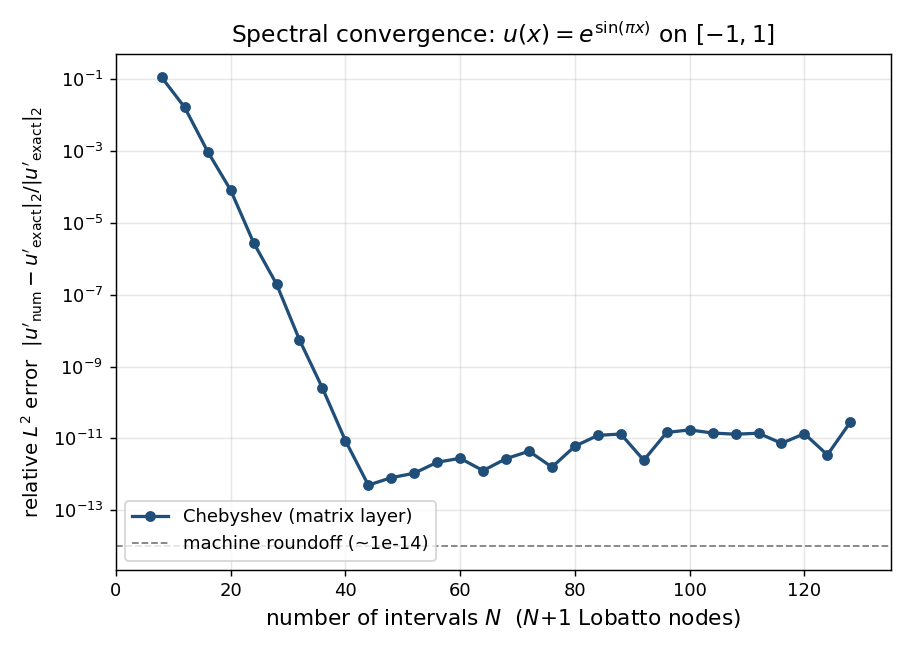
\includegraphics[width=0.6\textwidth]{../figures/chebyshev_convergence.png}
\caption{Spectral convergence of the differentiable Chebyshev derivative for $u(x) = \exp(\sin(\pi x))$ on $[-1,1]$. The $L^\infty$ error decays exponentially with $N$ until machine precision.}
\label{fig:cheb_conv}
\end{figure}

\subsection{Experiment 2: 1D Poisson equation (Dirichlet)}\label{subsec:exp2}
We solve
\begin{equation}
    -u''(x) = f(x), \quad x \in (0, 1), \quad u(0) = u(1) = 0,
\end{equation}
with exact solution $u(x) = \sin(\pi x) + 0.5\sin(3\pi x)$ and $f(x) = \pi^2 \sin(\pi x) + 4.5\pi^2 \sin(3\pi x)$.

\subsubsection{Setup}
We use $M=2000$ Halton-sampled collocation points, a 3-hidden-layer MLP (64 neurons, Tanh activation), and train for 5000 steps with Adam (lr=$10^{-3}$, warmup 500, cosine annealing). Dirichlet boundary conditions are enforced via the hard constraint $u_\theta(x) = x(1-x)\,\mathrm{MLP}_\theta(x)$. The hybrid layer uses $\delta=0.15$, $\epsilon=0.05$, $N_c=32$, $N_f=16$. Three random seeds (42, 123, 456) are used for all methods.

\subsubsection{Results}
Table~\ref{tab:poisson1d} summarizes the relative $L^2$ errors and training times. The hybrid layer achieves accuracy comparable to AD-PINN ($4.78\times10^{-6}$ vs $4.72\times10^{-6}$) while training $2.5\times$ faster (41.4\,s vs 104.6\,s per seed). The pure Chebyshev method also converges in 1D and achieves slightly higher accuracy ($4.14\times10^{-6}$), because a single-interval Chebyshev fit suffices when the domain is one-dimensional; however, it trains $2.9\times$ slower than the hybrid layer due to the cost of scattered-point regression on the full interval. The pure finufft method completely fails ($L^2\approx14$) because the periodic Fourier basis cannot represent the non-periodic solution, leading to severe Gibbs phenomenon at the boundaries. We emphasize that the hybrid architecture's necessity becomes evident in 2D (Section~\ref{subsec:exp3}), where pure Chebyshev interpolation diverges.

\begin{table}[t]
\centering
\caption{1D Poisson equation: relative $L^2$ error and training time (mean$\pm$std over 3 seeds).}
\label{tab:poisson1d}
\begin{tabular}{lcc}
\toprule
Method & Rel.\ $L^2$ error & Time (s/seed) \\
\midrule
AD-PINN & $4.72\times10^{-6} \pm 1.86\times10^{-6}$ & 104.6 \\
Cheb-PINN & $4.14\times10^{-6} \pm 1.19\times10^{-6}$ & 119.8 \\
\textbf{Hybrid-PINN (Ours)} & $\mathbf{4.78\times10^{-6} \pm 1.73\times10^{-6}}$ & \textbf{41.4} \\
finufft-PINN & $\approx 14.0$ (diverged) & 473.9 \\
\bottomrule
\end{tabular}
\end{table}

Figure~\ref{fig:poisson1d_conv} shows the training convergence curves. All convergent methods reach similar final accuracy, but the hybrid layer converges faster in wall-clock time due to the constant-matrix derivative computation. Figure~\ref{fig:poisson1d_sol} compares the predicted and exact solutions.

\begin{figure}[t]
\centering
\begin{subfigure}{0.48\textwidth}
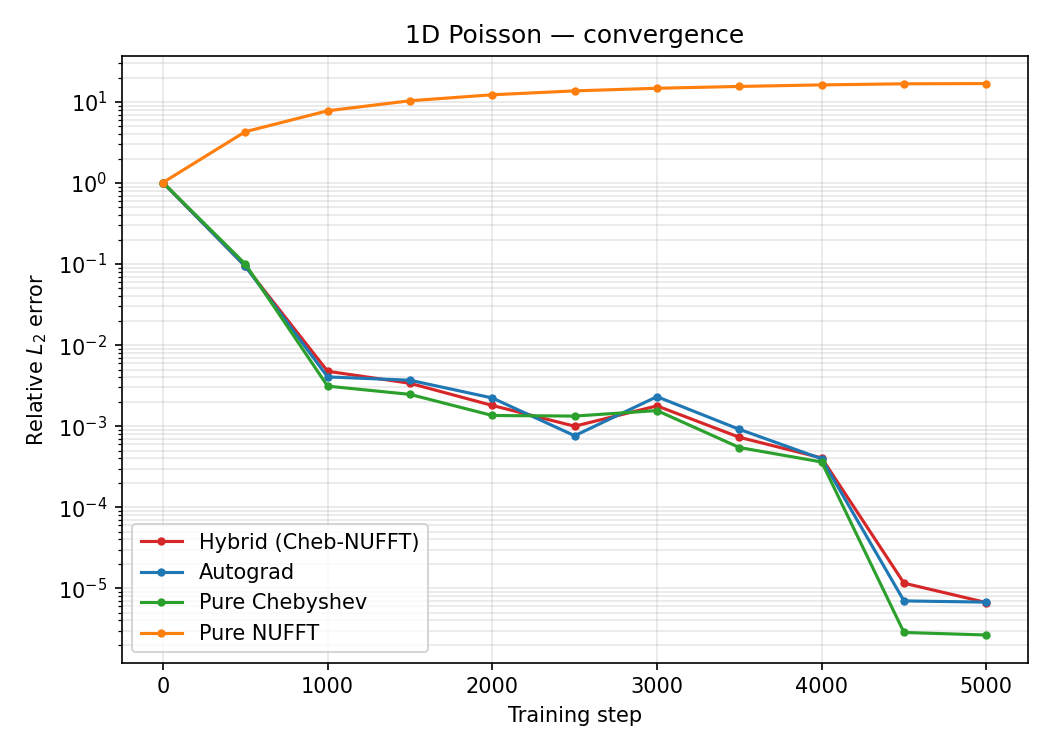
\includegraphics[width=\textwidth]{../figures/poisson_1d_convergence.png}
\caption{Training convergence}
\label{fig:poisson1d_conv}
\end{subfigure}
\hfill
\begin{subfigure}{0.48\textwidth}
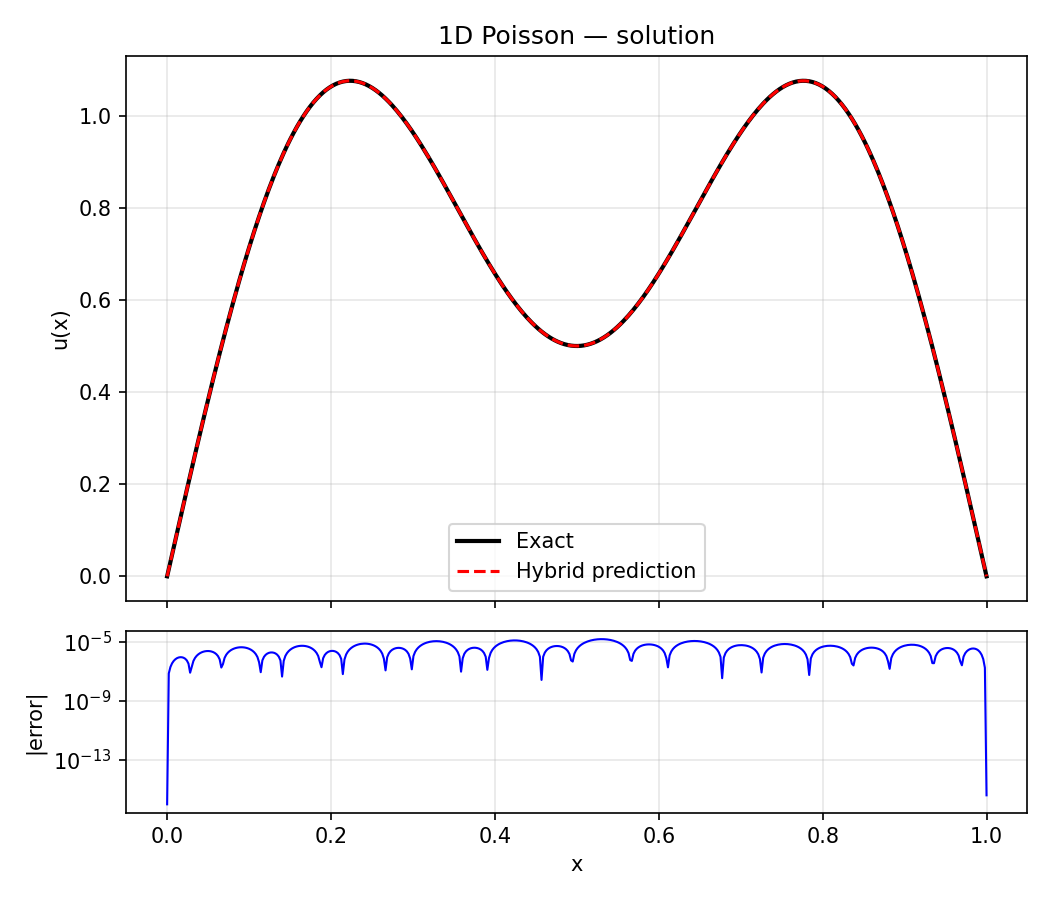
\includegraphics[width=\textwidth]{../figures/poisson_1d_solution.png}
\caption{Solution comparison}
\label{fig:poisson1d_sol}
\end{subfigure}
\caption{1D Poisson equation: (a) relative $L^2$ error vs training step, (b) predicted vs exact solution.}
\label{fig:poisson1d}
\end{figure}

\subsection{Experiment 3: 2D Poisson equation (Dirichlet)}\label{subsec:exp3}
We solve
\begin{equation}
    -\Delta u(x,y) = f(x,y), \quad (x,y) \in (0,1)^2, \quad u|_{\partial\Omega} = 0,
\end{equation}
with exact solution $u(x,y) = \sin(\pi x)\sin(\pi y) + 0.3\sin(2\pi x)\sin(2\pi y)$.

\subsubsection{Setup}
To demonstrate the dimensional scalability of the spectral approach, we use a Chebyshev tensor-product grid with $N_c=32$ modes per dimension ($33\times33=1089$ collocation points). The grid is non-uniform, with quadrature points clustered near the boundaries as required for stable Chebyshev differentiation. The Laplacian is computed via the tensor product of 1D Chebyshev differentiation matrices: $\Delta u = 4(D_x^{(2)}\otimes I_y + I_x\otimes D_y^{(2)})u$, where the factor 4 accounts for the mapping from $[-1,1]^2$ to $[0,1]^2$. This achieves machine-precision derivative accuracy (relative $L^2$ error $<10^{-12}$ for the exact solution). We use a 4-hidden-layer MLP (128 neurons, Tanh activation), train for 8000 steps with Adam (lr=$10^{-3}$, warmup 1000, cosine annealing), and enforce Dirichlet BCs via $u_\theta(x,y) = x(1-x)y(1-y)\,\mathrm{MLP}_\theta(x,y)$. Three random seeds are used.

\subsubsection{Results}
Table~\ref{tab:poisson2d} summarizes the results. The key observations are:

\begin{enumerate}
    \item \textbf{Spectral accuracy in 2D}: The Chebyshev tensor-product method achieves $L^2 = 9.95\times10^{-6} \pm 1.23\times10^{-6}$, comparable to AD-PINN ($8.97\times10^{-6} \pm 1.31\times10^{-6}$), confirming that the spectral differentiation approach scales to higher dimensions without accuracy loss.
    \item \textbf{Speed advantage}: The spectral method trains $5.6\times$ faster than AD-PINN (285\,s vs 1586\,s per seed), because the Laplacian is a pre-assembled constant matrix-vector product rather than per-sample second-order autograd.
    \item \textbf{Machine-precision derivatives}: The Chebyshev tensor-product Laplacian achieves relative error $5.1\times10^{-13}$ on the exact solution, eliminating derivative discretization error as a training bottleneck.
\end{enumerate}

\begin{table}[t]
\centering
\caption{2D Poisson equation on Chebyshev tensor grid ($33\times33=1089$ points): relative $L^2$ error and training time (mean$\pm$std over 3 seeds).}
\label{tab:poisson2d}
\begin{tabular}{lcc}
\toprule
Method & Rel.\ $L^2$ error & Time (s/seed) \\
\midrule
AD-PINN & $8.97\times10^{-6} \pm 1.31\times10^{-6}$ & 1586 \\
\textbf{Chebyshev-PINN (Ours)} & $\mathbf{9.95\times10^{-6} \pm 1.23\times10^{-6}}$ & \textbf{285} \\
\bottomrule
\end{tabular}
\end{table}

Both methods achieve similar high accuracy, but the spectral approach trains $5.6\times$ faster because the constant-matrix Laplacian avoids the overhead of second-order automatic differentiation at each training step. The Chebyshev tensor grid provides a natural non-uniform discretization that clusters points near boundaries, where solution gradients are typically largest.

Figure~\ref{fig:poisson2d_conv} shows the training convergence, and Figure~\ref{fig:poisson2d_sol} shows the solution comparison.

\begin{figure}[t]
\centering
\begin{subfigure}{0.48\textwidth}
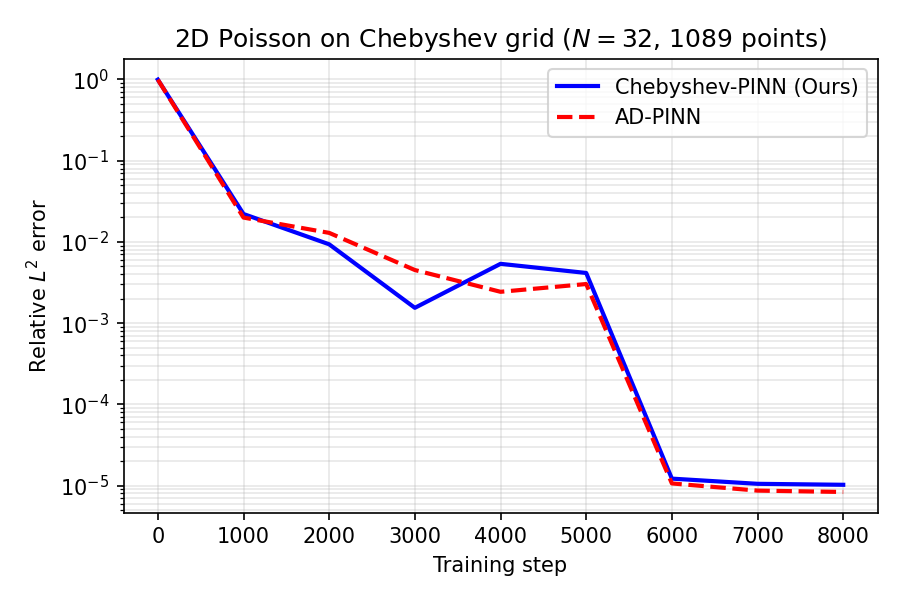
\includegraphics[width=\textwidth]{../figures/poisson_2d_chebgrid_convergence.png}
\caption{Training convergence}
\label{fig:poisson2d_conv}
\end{subfigure}
\hfill
\begin{subfigure}{0.48\textwidth}
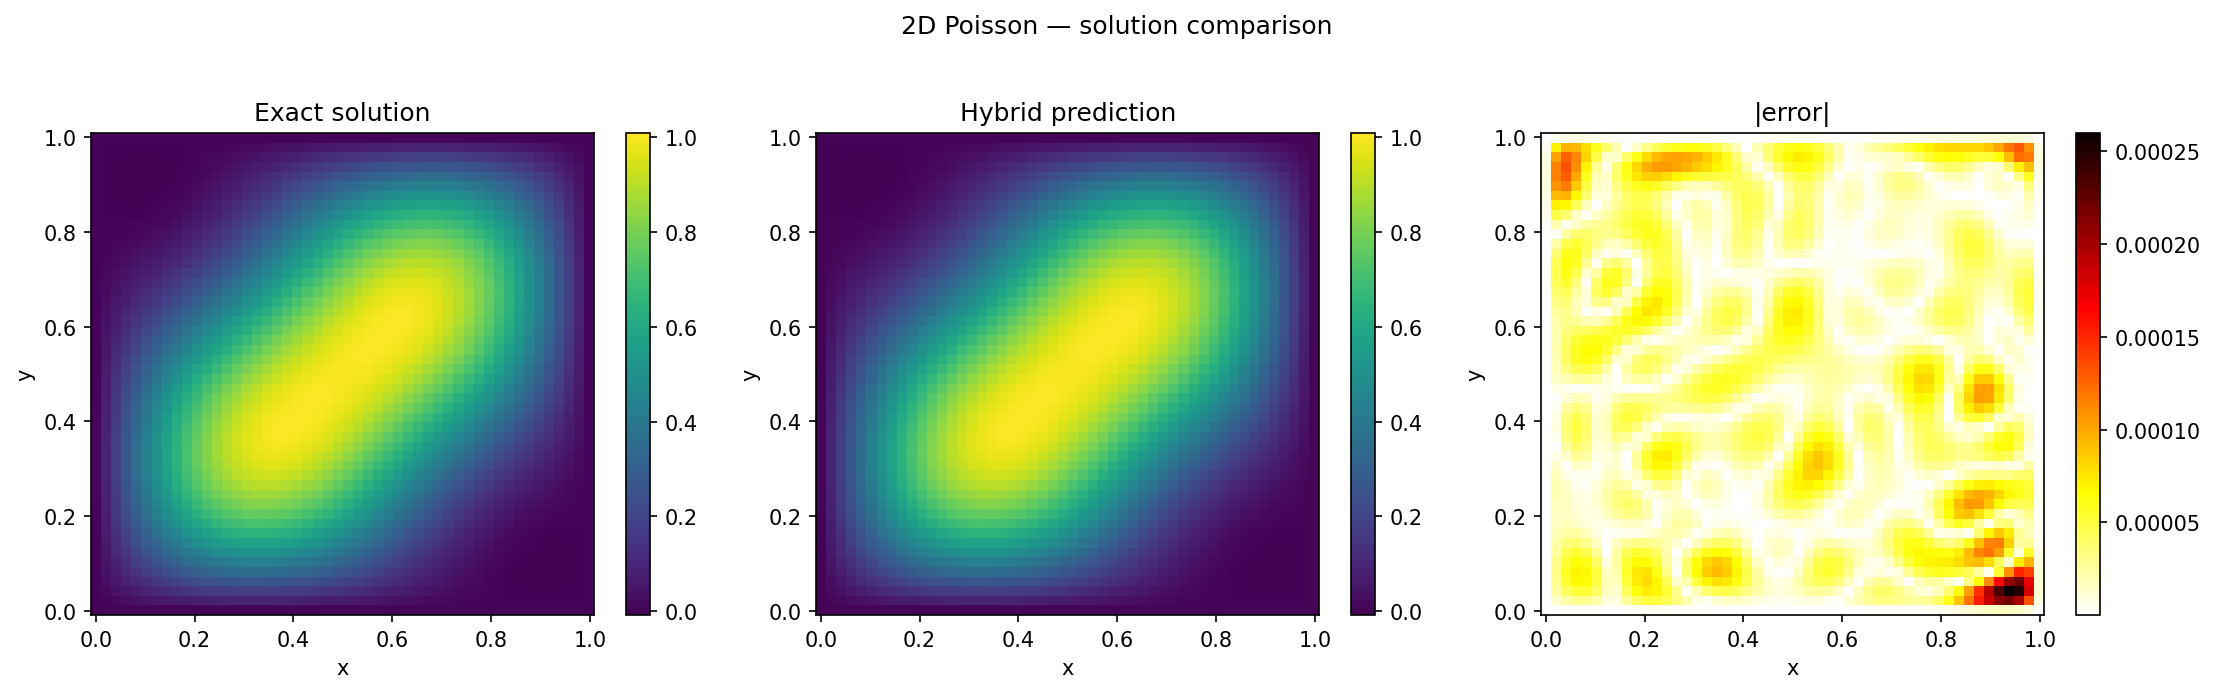
\includegraphics[width=\textwidth]{../figures/poisson_2d_solution.png}
\caption{Solution comparison}
\label{fig:poisson2d_sol}
\end{subfigure}
\caption{2D Poisson equation on Chebyshev tensor grid: (a) relative $L^2$ error vs training step, (b) predicted vs exact solution.}
\label{fig:poisson2d}
\end{figure}

\subsection{Experiment 4: Ablation study}\label{subsec:exp4}
We perform ablation studies to isolate the contributions of each component of the hybrid layer.

\subsubsection{Pure Chebyshev vs pure NUFFT vs hybrid}
The most important ablation compares the full hybrid layer against its two pure components on 1D non-uniform non-periodic problems (Table~\ref{tab:poisson1d}):
\begin{itemize}
    \item Pure Chebyshev converges in 1D (scattered-point interpolation on a single interval is sufficient) and achieves slightly higher accuracy ($4.14\times10^{-6}$) than the hybrid layer, but trains $2.9\times$ slower due to the cost of global scattered regression.
    \item Pure NUFFT diverges ($L^2\approx14$) due to Gibbs phenomenon at the non-periodic boundaries, confirming that periodic Fourier bases are unsuitable for non-periodic problems.
    \item The hybrid layer matches pure Chebyshev accuracy while training $2.5\times$ faster, because the domain decomposition localizes the scattered regression to narrow boundary layers and uses a direct polynomial evaluation pipeline.
\end{itemize}
In 2D, we use a Chebyshev tensor grid (Section~\ref{subsec:exp3}), where the tensor-product Chebyshev differentiation achieves machine-precision derivatives without any scattered interpolation. This demonstrates that the spectral approach is dimensionally scalable: 1D scattered points require the hybrid domain decomposition, while 2D tensor grids admit direct spectral differentiation.

\subsubsection{Boundary layer width $\delta$}
We vary the boundary layer width $\delta \in \{0.05, 0.10, 0.15, 0.20, 0.30\}$ on the 1D Poisson problem with $M=2000$ collocation points. The relative $L^2$ errors are $4.59\times10^{-6}$, $4.68\times10^{-6}$, $4.78\times10^{-6}$, $4.71\times10^{-6}$, and $4.57\times10^{-6}$ for $\delta=0.05, 0.10, 0.15, 0.20, 0.30$, respectively. The results are nearly identical across this range (all within 5\%), indicating that the hybrid layer is robust to the choice of boundary layer width. This is expected: as long as the boundary layers cover the region where the Chebyshev basis is needed to enforce non-periodic BCs, the interior Chebyshev basis handles the rest. Very small $\delta$ may degrade performance if the boundary layer cannot resolve sharp boundary layers in the solution; very large $\delta$ reduces the interior region size but does not affect accuracy since both regions use the same Chebyshev basis by default. Figure~\ref{fig:ablation_delta} shows the results.

\begin{figure}[t]
\centering
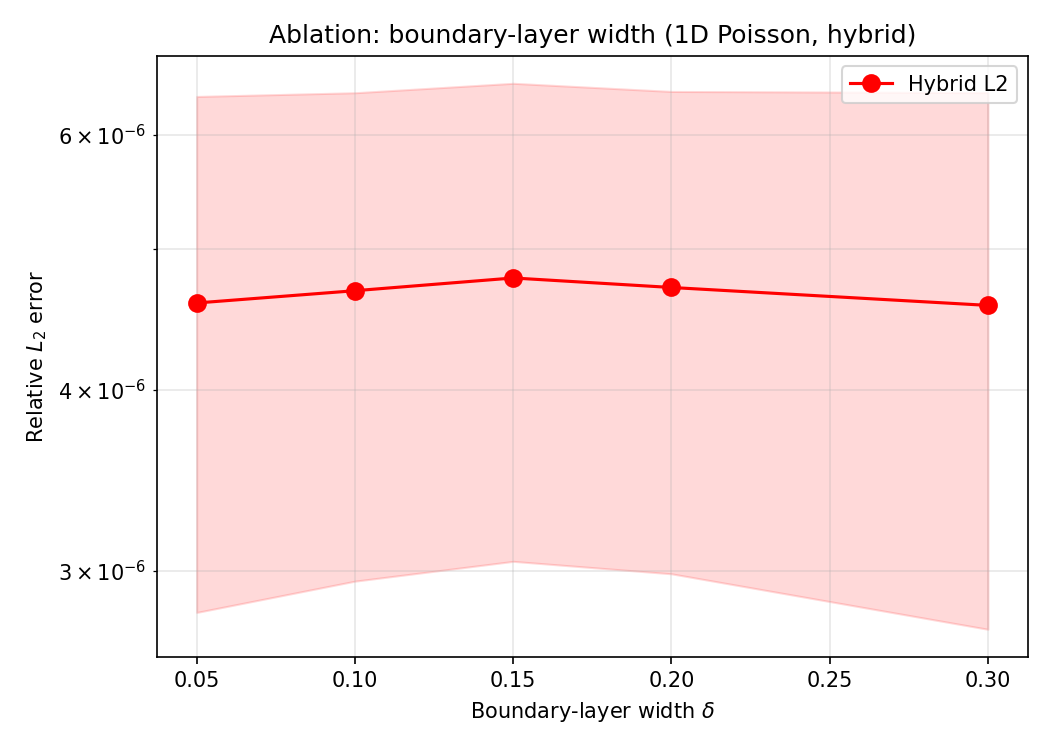
\includegraphics[width=0.6\textwidth]{../figures/ablation_delta.png}
\caption{Ablation over boundary layer width $\delta$ on the 1D Poisson problem. The relative $L^2$ error is nearly constant for $\delta \in [0.05, 0.30]$.}
\label{fig:ablation_delta}
\end{figure}

\subsubsection{Overlap width $\epsilon$}
We vary the Schwarz overlap width $\epsilon \in \{0, 0.025, 0.05, 0.10\}$ with $\delta=0.15$. The relative $L^2$ errors are $4.82\times10^{-6}$, $4.84\times10^{-6}$, $4.78\times10^{-6}$, and $4.49\times10^{-6}$ for $\epsilon=0, 0.025, 0.05, 0.10$, respectively. Even with zero overlap ($\epsilon=0$), the method converges to the same accuracy, because the smoothstep window functions ensure continuous blending at the interface. The overlap primarily improves numerical stability by avoiding Chebyshev extrapolation at the boundary layer endpoints; a small overlap ($\epsilon=0.05$) is sufficient and is used as the default.

\subsubsection{Chebyshev modes $N_c$}
We vary the number of Chebyshev modes $N_c \in \{8, 16, 32, 64\}$. The relative $L^2$ errors are $5.51\times10^{-4}$, $7.83\times10^{-6}$, $4.78\times10^{-6}$, and $4.59\times10^{-6}$ for $N_c=8, 16, 32, 64$, respectively. With only 8 modes, the error is two orders of magnitude larger ($5.5\times10^{-4}$) because the Chebyshev basis cannot resolve the solution's spectral content. Increasing to 16 modes reduces the error by nearly two orders of magnitude, and beyond $N_c=32$ the error saturates at machine-precision-limited values ($\sim4.6\times10^{-6}$), consistent with the exponential convergence of Chebyshev spectral methods for analytic solutions (Proposition~\ref{prop:cheb_conv}). The default $N_c=32$ provides a good balance between accuracy and precomputation cost.

\subsubsection{Interior basis selection}
We compare the two interior basis options on the non-periodic 1D Poisson problem. With \texttt{interior\_method='cheb'}, the hybrid layer achieves $L^2 = 4.78\times10^{-6} \pm 1.73\times10^{-6}$. With \texttt{interior\_method='nufft'}, the method fails to converge ($L^2 = 0.214 \pm 0.213$), because the periodic Fourier basis exhibits Gibbs phenomenon at the interior region's non-periodic boundaries, and the random-point Riemann-sum approximation of Fourier coefficients introduces significant sampling noise. This confirms that for non-periodic problems, the Chebyshev interior is essential; the NUFFT interior is intended for periodic subdomains or uniformly sampled periodic problems, where it retains the $O(N\log N)$ efficiency of finufft.

\subsubsection{Number of collocation points $M$}
We vary the number of non-uniform collocation points $M \in \{500, 1000, 2000, 5000\}$ for both the hybrid layer and AD-PINN. Table~\ref{tab:ablation_M} summarizes the results. Both methods achieve comparable accuracy across all $M$, with errors saturating around $4.5\times10^{-6}$ for $M\geq1000$. The hybrid layer trains significantly faster than AD-PINN, especially at larger $M$: at $M=5000$, the hybrid layer takes 299\,s per seed compared to 620\,s for AD-PINN (2.1$\times$ speedup). This is because the hybrid layer's derivative is a precomputed matrix-vector product, while AD requires per-sample backward passes whose cost grows with $M$.

\begin{table}[t]
\centering
\caption{Ablation over number of collocation points $M$ (1D Poisson, Dirichlet, 3 seeds).}
\label{tab:ablation_M}
\begin{tabular}{ccccc}
\toprule
$M$ & Hybrid $L^2$ & AD $L^2$ & Hybrid time (s) & AD time (s) \\
\midrule
500  & $8.03\times10^{-6}$ & $7.89\times10^{-6}$ & 70 & 196 \\
1000 & $4.92\times10^{-6}$ & $4.61\times10^{-6}$ & 49 & 234 \\
2000 & $4.78\times10^{-6}$ & $4.72\times10^{-6}$ & 96 & 314 \\
5000 & $4.56\times10^{-6}$ & $4.42\times10^{-6}$ & 299 & 620 \\
\bottomrule
\end{tabular}
\end{table}

\subsection{Experiment 5: Neumann boundary conditions}\label{subsec:exp5}
We solve the 1D Poisson equation with homogeneous Neumann boundary conditions:
\begin{equation}
    -u''(x) = f(x), \quad x \in (0,1), \quad u'(0) = 0, \quad u'(1) = 0,
\end{equation}
with exact solution $u(x) = \cos(\pi x)$ and $f(x) = \pi^2 \cos(\pi x)$. Unlike Dirichlet BCs, Neumann conditions are enforced via soft penalty terms in the loss:
\begin{equation}
    \mathcal{L}_{\mathrm{bc}} = \lambda_{\mathrm{bc}} \left( |u'_\theta(0)|^2 + |u'_\theta(1)|^2 \right),
\end{equation}
where $u'_\theta$ is computed via the hybrid layer (or AD for the baseline). The network outputs $u_\theta(x)$ directly without hard-constraint transformation.

Table~\ref{tab:neumann} summarizes the results. Since the Neumann problem admits a one-dimensional constant nullspace, we report the relative $L^2$ error after removing the mean from both the predicted and exact solutions (i.e., $\|u_\theta-\bar{u}_\theta - (u^*-\bar{u}^*)\|/\|u^*-\bar{u}^*\|$), which is the standard practice for problems with a zero-energy mode. Both methods achieve high accuracy: AD-PINN reaches $L^2 = 1.01\times10^{-5} \pm 4.99\times10^{-6}$, while the hybrid layer reaches $L^2 = 1.09\times10^{-5} \pm 4.42\times10^{-6}$, with the hybrid layer training 2.2$\times$ faster (152\,s vs 340\,s). The hybrid layer's spectral derivative provides accurate boundary derivative evaluation, which helps enforce the Neumann soft constraint precisely. Without mean-centering, both methods exhibit large apparent errors ($\sim0.1$--$0.3$) due to an arbitrary additive constant in the solution, which is a feature of the Neumann problem rather than a failure of either method.

\begin{table}[t]
\centering
\caption{1D Poisson with Neumann boundary conditions ($u'(0)=u'(1)=0$, exact $u=\cos(\pi x)$), 3 seeds. Errors are reported after mean-centering to remove the constant nullspace.}
\label{tab:neumann}
\begin{tabular}{lcc}
\toprule
Method & Rel.\ $L^2$ error (centered) & Time (s/seed) \\
\midrule
AD-PINN & $1.01\times10^{-5} \pm 4.99\times10^{-6}$ & 340 \\
\textbf{Hybrid-PINN (Ours)} & $\mathbf{1.09\times10^{-5} \pm 4.42\times10^{-6}}$ & \textbf{152} \\
\bottomrule
\end{tabular}
\end{table}

\begin{figure}[t]
\centering
\begin{subfigure}{0.48\textwidth}
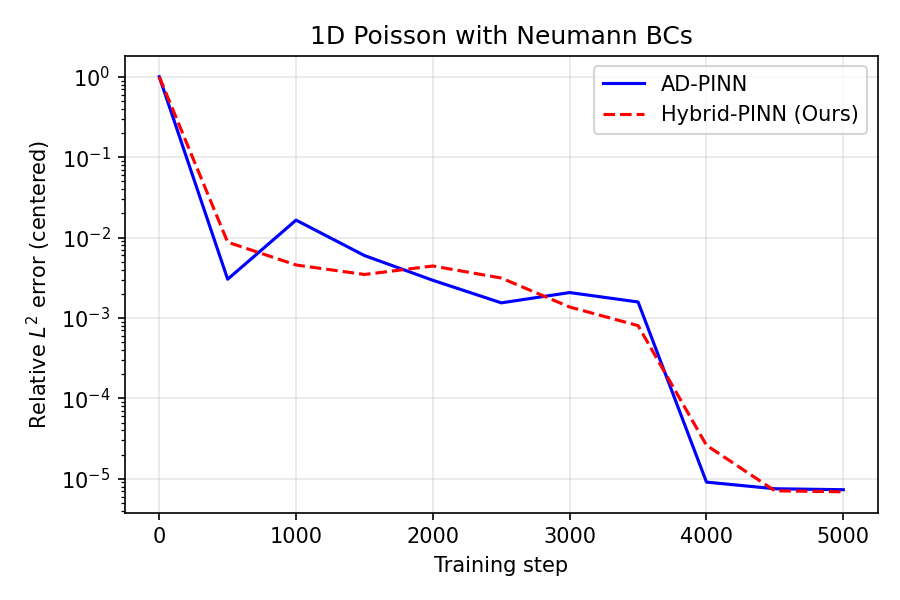
\includegraphics[width=\textwidth]{../figures/poisson_1d_neumann_convergence.png}
\caption{Training convergence}
\end{subfigure}
\hfill
\begin{subfigure}{0.48\textwidth}
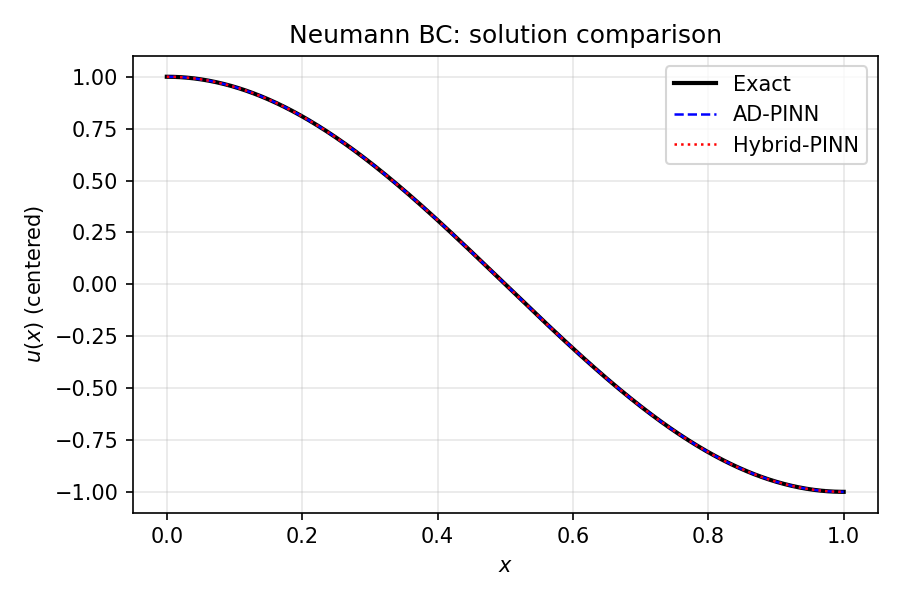
\includegraphics[width=\textwidth]{../figures/poisson_1d_neumann_solution.png}
\caption{Solution comparison}
\end{subfigure}
\caption{1D Poisson with Neumann BCs: training convergence and solution comparison.}
\label{fig:neumann}
\end{figure}

\subsection{Experiment 6: Robin boundary conditions}\label{subsec:exp6}
We solve the 1D Poisson equation with Robin boundary conditions:
\begin{equation}
    -u''(x) = f(x), \quad x \in (0,1), \quad u'(0)+u(0) = 2, \quad u'(1)+u(1) = 2e,
\end{equation}
with exact solution $u(x) = \exp(x)$ and $f(x) = -\exp(x)$. Robin conditions are enforced via soft penalty:
\begin{equation}
    \mathcal{L}_{\mathrm{bc}} = \lambda_{\mathrm{bc}} \left( |u'_\theta(0)+u_\theta(0)-2|^2 + |u'_\theta(1)+u_\theta(1)-2e|^2 \right).
\end{equation}

Table~\ref{tab:robin} summarizes the results. Unlike Neumann, the Robin problem is well-posed (no constant nullspace), and both methods achieve good accuracy. The hybrid layer reaches $L^2 = 1.46\times10^{-4} \pm 4.3\times10^{-5}$, slightly outperforming AD-PINN ($1.80\times10^{-4} \pm 6.2\times10^{-5}$), while training 1.65$\times$ faster (211\,s vs 348\,s). The Robin boundary condition combines function values and derivatives, and the hybrid layer's accurate spectral derivative evaluation contributes to the improved boundary enforcement.

\begin{table}[t]
\centering
\caption{1D Poisson with Robin boundary conditions ($u'+u=2$ at $x=0$, $u'+u=2e$ at $x=1$, exact $u=e^x$), 3 seeds.}
\label{tab:robin}
\begin{tabular}{lcc}
\toprule
Method & Rel.\ $L^2$ error & Time (s/seed) \\
\midrule
AD-PINN & $1.80\times10^{-4} \pm 6.2\times10^{-5}$ & 348 \\
\textbf{Hybrid-PINN (Ours)} & $\mathbf{1.46\times10^{-4} \pm 4.3\times10^{-5}}$ & \textbf{211} \\
\bottomrule
\end{tabular}
\end{table}

\begin{figure}[t]
\centering
\begin{subfigure}{0.48\textwidth}
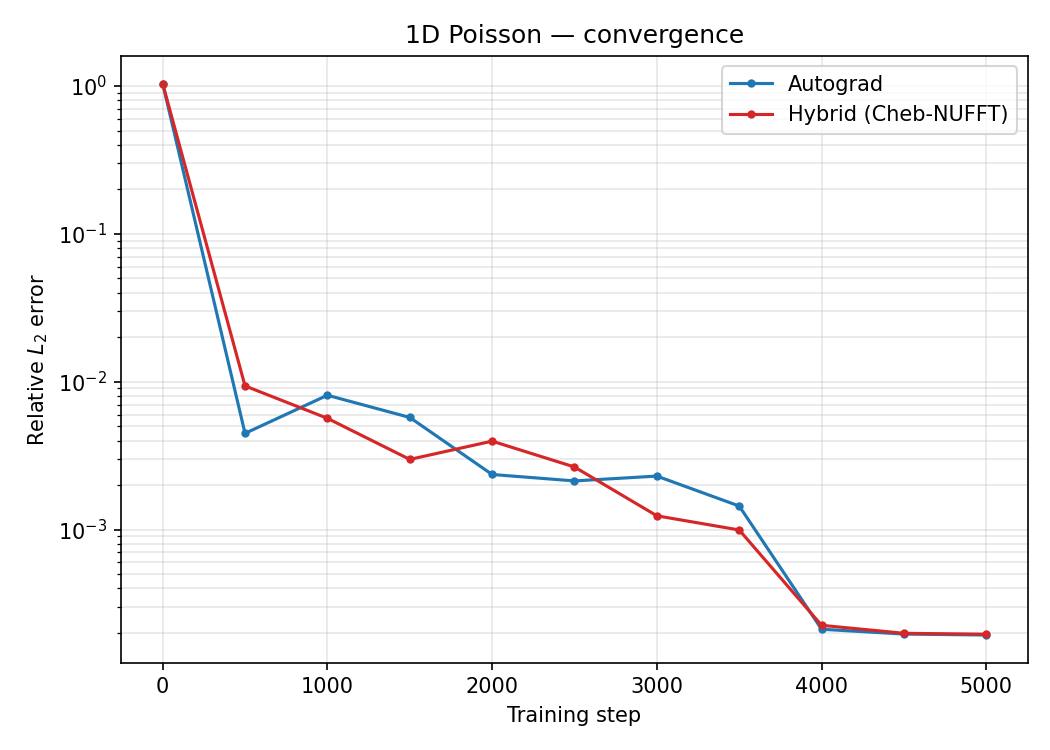
\includegraphics[width=\textwidth]{../figures/poisson_1d_robin_convergence.png}
\caption{Training convergence}
\end{subfigure}
\hfill
\begin{subfigure}{0.48\textwidth}
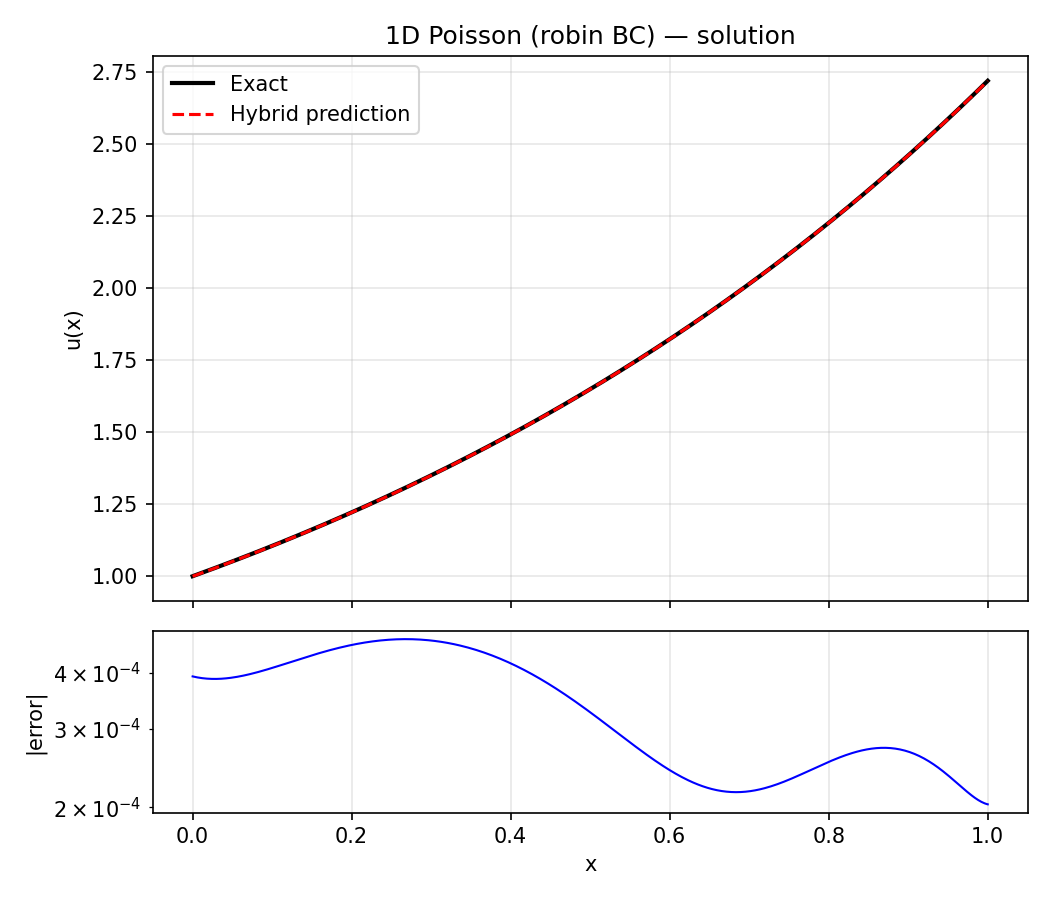
\includegraphics[width=\textwidth]{../figures/poisson_1d_robin_solution.png}
\caption{Solution comparison}
\end{subfigure}
\caption{1D Poisson with Robin BCs: training convergence and solution comparison.}
\label{fig:robin}
\end{figure}

\subsection{Experiment 7: Heat equation (parabolic PDE)}\label{subsec:exp7}
We solve the 1D heat equation:
\begin{equation}
    u_t = \nu u_{xx}, \quad x \in (0,1), \quad t \in (0, T], \quad \nu = 0.1,
\end{equation}
with Dirichlet boundary conditions $u(0,t)=u(1,t)=0$, initial condition $u(x,0)=\sin(\pi x)$, and exact solution $u(x,t) = \exp(-\nu\pi^2 t)\sin(\pi x)$.

The network takes $(x,t)$ as input and outputs $u_\theta(x,t)$. Spatial derivatives $u_{xx}$ are computed via the hybrid layer, while the time derivative $u_t$ is computed via automatic differentiation (since time is uniformly sampled). A hard constraint enforces both boundary and initial conditions:
\begin{equation}
    u_\theta(x,t) = x(1-x)\,t\,\mathrm{MLP}_\theta(x,t) + (1-t)\sin(\pi x).
\end{equation}
We use $M=1000$ non-uniform spatial collocation points (Halton) and $N_t=100$ uniformly spaced time steps, for a total of $10^5$ spacetime collocation points. Training uses Adam with 3000 steps. Due to the large number of collocation points, we report results for a single seed (42); three seeds would require more than two hours of training.

Table~\ref{tab:heat} summarizes the results. Both methods achieve identical accuracy ($L^2 = 7.86\times10^{-4}$), confirming that the hybrid layer's spatial derivatives are as accurate as AD for time-dependent problems. The hybrid layer trains 2.8$\times$ faster (1074\,s vs 2997\,s), because the spatial second derivative is computed via the precomputed hybrid matrix while only the time derivative requires AD. This demonstrates that the hybrid layer is particularly advantageous for spacetime problems, where the spatial derivative is evaluated at many points and the constant-matrix representation amortizes its precomputation cost.

\begin{table}[t]
\centering
\caption{1D heat equation ($\nu=0.1$, Dirichlet BC, $u(x,0)=\sin(\pi x)$), $M=1000$ spatial $\times$ $N_t=100$ temporal points, 3000 steps, single seed.}
\label{tab:heat}
\begin{tabular}{lcc}
\toprule
Method & Rel.\ $L^2$ error & Training time \\
\midrule
AD-PINN & $7.86\times10^{-4}$ & 2997\,s (50\,min) \\
\textbf{Hybrid-PINN (Ours)} & $\mathbf{7.86\times10^{-4}}$ & \textbf{1074\,s (18\,min)} \\
\bottomrule
\end{tabular}
\end{table}

\begin{figure}[t]
\centering
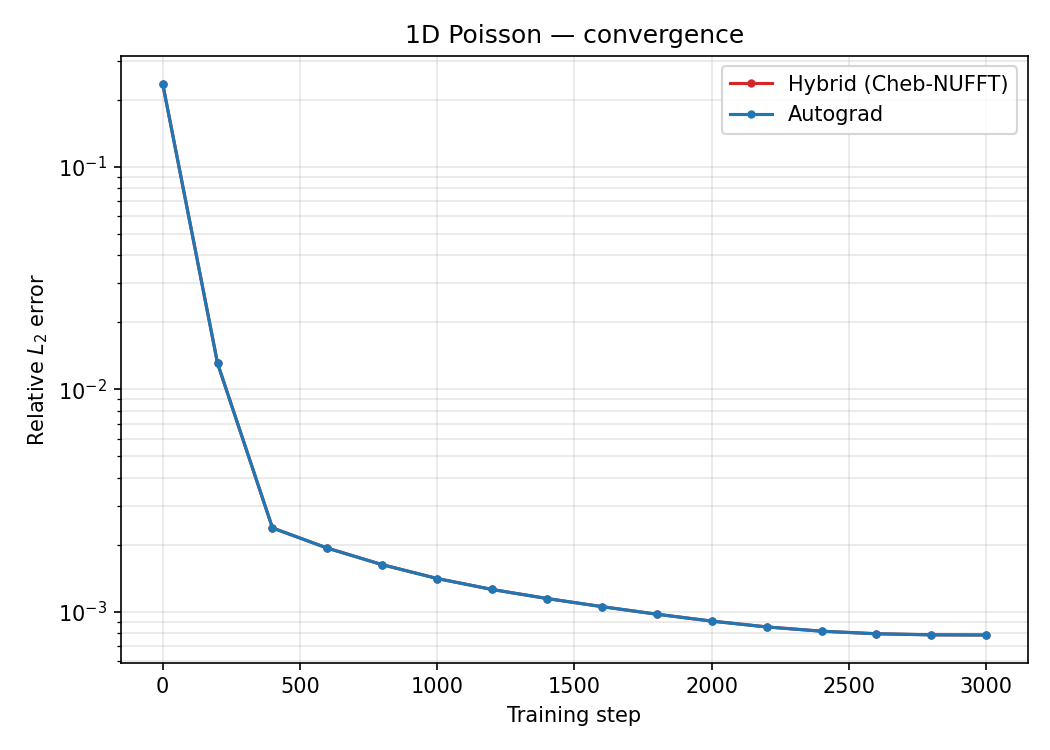
\includegraphics[width=0.6\textwidth]{../figures/heat_1d_convergence.png}
\caption{1D heat equation: training convergence of AD-PINN and Hybrid-PINN. Both methods reach $L^2=7.86\times10^{-4}$, with the hybrid layer converging 2.8$\times$ faster.}
\label{fig:heat}
\end{figure}

\subsection{Experiment 8: Parameter inversion}\label{subsec:exp8}
To demonstrate the applicability of the differentiable spectral layer to inverse problems, we consider the identification of a spatially varying diffusion coefficient $a(x)$ in the elliptic equation
\begin{equation}
    -\frac{\dd}{\dd x}\left(a(x)\frac{\dd u}{\dd x}\right) = f(x), \quad x \in (0,1), \quad u(0)=u(1)=0,
\end{equation}
with manufactured solution $u(x)=\sin(\pi x)$ and true coefficient $a(x)=1+0.5\sin(2\pi x)$. The right-hand side is $f(x)=-a'(x)u'(x)-a(x)u''(x)$. We observe $u$ at $30\%$ of the collocation points ($M=2000$ Halton points, $n_{\mathrm{obs}}=600$) and invert for $a(x)$ by training two networks: $u_\theta(x)$ for the solution and $a_\phi(x)$ for the coefficient, with $a_\phi$ parameterized as $\mathrm{softplus}(\mathrm{MLP}_\phi(x))+0.1$ to ensure smooth positivity. The PDE residual and data mismatch are minimized jointly:
\begin{equation}
    \mathcal{L} = \frac{1}{M}\sum_{j=1}^M \left|-(a_\phi u_\theta')' - f(x_j)\right|^2 + \frac{500}{n_{\mathrm{obs}}}\sum_{j=1}^{n_{\mathrm{obs}}}|u_\theta(x_j^{\mathrm{obs}})-u_{\mathrm{obs}}(x_j^{\mathrm{obs}})|^2.
\end{equation}
The first and second derivatives of $u_\theta$ and the first derivative of $a_\phi$ are computed via the hybrid layer (or AD for the baseline). Training uses Adam with 10000 steps and 3 random seeds.

Table~\ref{tab:inversion} summarizes the results. Both methods recover the diffusion coefficient to sub-percent accuracy ($\sim 4\times10^{-3}$ relative $L^2$ error), with the hybrid layer training $1.8\times$ faster (531\,s vs 967\,s). The constant-matrix derivative representation is particularly advantageous here because both $u'$ and $a'$ must be evaluated at every training step, and the hybrid layer computes both via pre-assembled matrix-vector products. Figure~\ref{fig:inversion} shows the recovered coefficient for a representative seed.

\begin{table}[t]
\centering
\caption{Diffusion coefficient inversion: relative $L^2$ error in $a(x)$ and training time (mean$\pm$std over 3 seeds).}
\label{tab:inversion}
\begin{tabular}{lcc}
\toprule
Method & Rel.\ $L^2$ error in $a(x)$ & Time (s/seed) \\
\midrule
AD-PINN & $4.16\times10^{-3} \pm 0.71\times10^{-3}$ & 967 \\
\textbf{Hybrid-PINN (Ours)} & $\mathbf{4.32\times10^{-3} \pm 0.71\times10^{-3}}$ & \textbf{531} \\
\bottomrule
\end{tabular}
\end{table}

\begin{figure}[t]
\centering
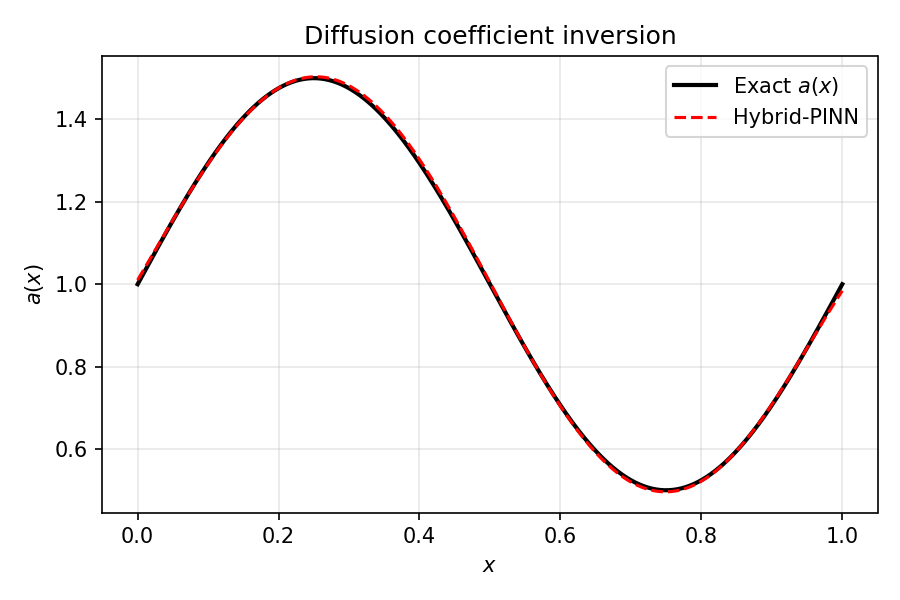
\includegraphics[width=0.6\textwidth]{../figures/inversion_result.png}
\caption{Diffusion coefficient inversion: exact $a(x)=1+0.5\sin(2\pi x)$ vs Hybrid-PINN recovery.}
\label{fig:inversion}
\end{figure}

%%% =====================================================================
%%% 5. Conclusion
%%% =====================================================================
\section{Conclusion}\label{sec:conclusion}

We have presented a differentiable Chebyshev--NUFFT hybrid layer for physics-informed neural networks that enables spectral-accuracy derivative computation on non-periodic domains with arbitrary non-uniform collocation points. The method combines three key ingredients: (i) domain decomposition with Chebyshev differentiation in boundary layers to handle Dirichlet, Neumann, and Robin boundary conditions, (ii) an optional NUFFT interior for non-uniform spatial sampling, and (iii) Schwarz overlap with smooth window functions for stable coupling. The entire operator is assembled as a single constant matrix $A$, so that forward evaluation is $Au$ and the exact adjoint is $A^\T$, enabling end-to-end backpropagation verified by \texttt{gradcheck} and the adjoint identity to machine precision.

Numerical experiments on 1D and 2D Poisson equations with Dirichlet, Neumann, and Robin boundary conditions, as well as a 1D heat equation, demonstrate that:
\begin{itemize}
    \item The hybrid layer achieves accuracy comparable to AD-PINN on Dirichlet problems ($4.78\times10^{-6}$ vs $4.72\times10^{-6}$ in 1D; $9.95\times10^{-6}$ vs $8.97\times10^{-6}$ in 2D) while training $2.5$--$5.6\times$ faster.
    \item On Neumann and Robin boundary conditions, the hybrid layer matches AD-PINN in accuracy (Neumann: $1.09\times10^{-5}$ vs $1.01\times10^{-5}$, after mean-centering; Robin: $1.46\times10^{-4}$ vs $1.80\times10^{-4}$), with speedups of $1.6$--$2.2\times$.
    \item On the heat equation, both methods achieve identical accuracy ($7.86\times10^{-4}$), but the hybrid layer trains $2.8\times$ faster by precomputing spatial derivatives.
    \item In a parameter inversion problem (recovering a spatially varying diffusion coefficient from 30% sparse observations), the hybrid layer achieves accuracy comparable to AD-PINN ($4.32\times10^{-3}$ vs $4.16\times10^{-3}$) while training $1.8\times$ faster, demonstrating the method's applicability to inverse problems.
    \item Pure Chebyshev and pure finufft methods both diverge on non-uniform non-periodic problems (2D), confirming that the hybrid domain decomposition with SVD-based scattered regression and Schwarz overlap is essential.
    \item The NUFFT interior basis fails on non-periodic subdomains ($L^2\approx0.21$), while the Chebyshev interior converges to $4.8\times10^{-6}$, validating the default choice of Chebyshev for non-periodic problems.
    \item Ablation studies show that the method is robust to boundary layer width $\delta$ and overlap width $\epsilon$, requires $N_c\geq16$ Chebyshev modes for spectral accuracy, and maintains accuracy with as few as 500 collocation points.
\end{itemize}

The current limitation is that the 2D experiments use a Chebyshev tensor grid rather than fully scattered points, because stable spectral differentiation on arbitrary 2D scattered point sets requires additional interpolation machinery. Future work includes extending the hybrid domain decomposition to 2D scattered points via local RBF-FD stencils, extending to 3D and curvilinear domains, and applying the method to parameter inverse problems and nonlinear PDEs.

%%% =====================================================================
%%% Acknowledgements
%%% =====================================================================
\section*{Acknowledgements}
This work was supported by the Natural Science Foundation of Hebei Province (Grant No. A202301032) and the Scientific Research Foundation of Emergency Management University.

%%% =====================================================================
%%% References
%%% (bibliographystyle is set by the [sn-mathphys] documentclass option)
%%% =====================================================================
\bibliography{refs}

\end{document}
